\documentclass[a4paper,12pt]{article}

%%% Работа с русским языком
\usepackage{cmap}					% поиск в PDF
\usepackage{mathtext} 				% русские буквы в формулах
\usepackage[T2A]{fontenc}			% кодировка
\usepackage[utf8]{inputenc}			% кодировка исходного текста
\usepackage[english,russian]{babel}	% локализация и переносы
\usepackage{xcolor}
\usepackage{hyperref}
 % Цвета для гиперссылок
\definecolor{linkcolor}{HTML}{799B03} % цвет ссылок
\definecolor{urlcolor}{HTML}{799B03} % цвет гиперссылок

\hypersetup{pdfstartview=FitH,  linkcolor=linkcolor,urlcolor=urlcolor, colorlinks=true}

%%% Дополнительная работа с математикой
\usepackage{amsfonts,amssymb,amsthm,mathtools} % AMS
\usepackage{amsmath}
\usepackage{icomma} % "Умная" запятая: $0,2$ --- число, $0, 2$ --- перечисление

%% Номера формул
%\mathtoolsset{showonlyrefs=true} % Показывать номера только у тех формул, на которые есть \eqref{} в тексте.

%% Шрифты
\usepackage{euscript}	 % Шрифт Евклид
\usepackage{mathrsfs} % Красивый матшрифт

%% Свои команды
\DeclareMathOperator{\sgn}{\mathop{sgn}}

%% Перенос знаков в формулах (по Львовскому)
\newcommand*{\hm}[1]{#1\nobreak\discretionary{}
{\hbox{$\mathsurround=0pt #1$}}{}}
% графика
\usepackage{graphicx}
\graphicspath{{pictures/}}
\DeclareGraphicsExtensions{.pdf,.png,.jpg}
\author{Бурмашев Григорий, БПМИ-208}
\title{ТВиМС, дз какое-то}
\date{\today}
\begin{document}
\maketitle
\section*{Номер 1}
Ну, нужно найти мат.ожидания, так что ищем их, для этого надо выразить плотности, выражаем (берем с сема, хех):
\[
\rho_{X_{(n)}} (t) = 
I_{[a, b]}
\cdot \frac{n \cdot (t - a)^{n - 1}}{(b - a)^n}
\]
\[
\rho_{X_{(1)}} (t) =I_{[a, b]} \cdot  \frac{n \cdot (b - t)^{n - 1}}{(b - a)^n}
\]
Тогда:
\[
\mathbb{E}\left[
X_{(n)}
\right] = \int\limits_a^b  t \cdot
 \frac{n \cdot (t - a)^{n - 1}}{(b - a)^n} dt = \frac{n}{(b - a)^n} \int\limits_a^b (t - a)^n dt + \frac{na}{(b - a)^n} \int\limits_a^b (t - a)^{n - 1} dt = \frac{a + bn }{n + 1}
\]
А для $X_{(1)}$:
\[
\mathbb{E} \left[
X_{(1)}
\right]
=
\int\limits_a^b  t  \cdot  \frac{n \cdot (b - t)^{n - 1}}{(b - a)^n}dt = n \cdot  \int\limits_a^b  \frac{(t -b )(b -t)^{n - 1}}{(b - a)^n } dt + nb \int\limits_a^b \frac{(b - t)^{n - 1}}{(b -a)^n} dt =  \frac{an + b}{n + 1}
\]
Тогда мат.ожидание:
\[
\mathbb{E} \left( \frac{X_{(1)} + X_{(n)}}{2} \right) = \frac{1}{2} \mathbb{E} X_{(1)} + \frac{1}{2} \mathbb{E}X_{(n)} = 
\frac{1}{2} \cdot  \frac{an + b}{n + 1} + \frac{1}{2} \cdot \frac{a + bn }{n + 1} = \frac{a + b}{2} = \theta 
\]
А значит несмещенность есть
\begin{center}
\textbf{Ответ: } несмещенность есть
\end{center}
\clearpage
\section*{Номер 2}
Задача 1 в 1 с сема, только другой $n$, буду вставлять куски с семинара Зеленова, чтобы не делать одно и тоже.
\\
Хотим доказать, что:
\[
X_{(m + 1) } \overset{P}{\longrightarrow} x_{\frac12}, \; n = 2m \rightarrow \infty 
\]
\begin{center}
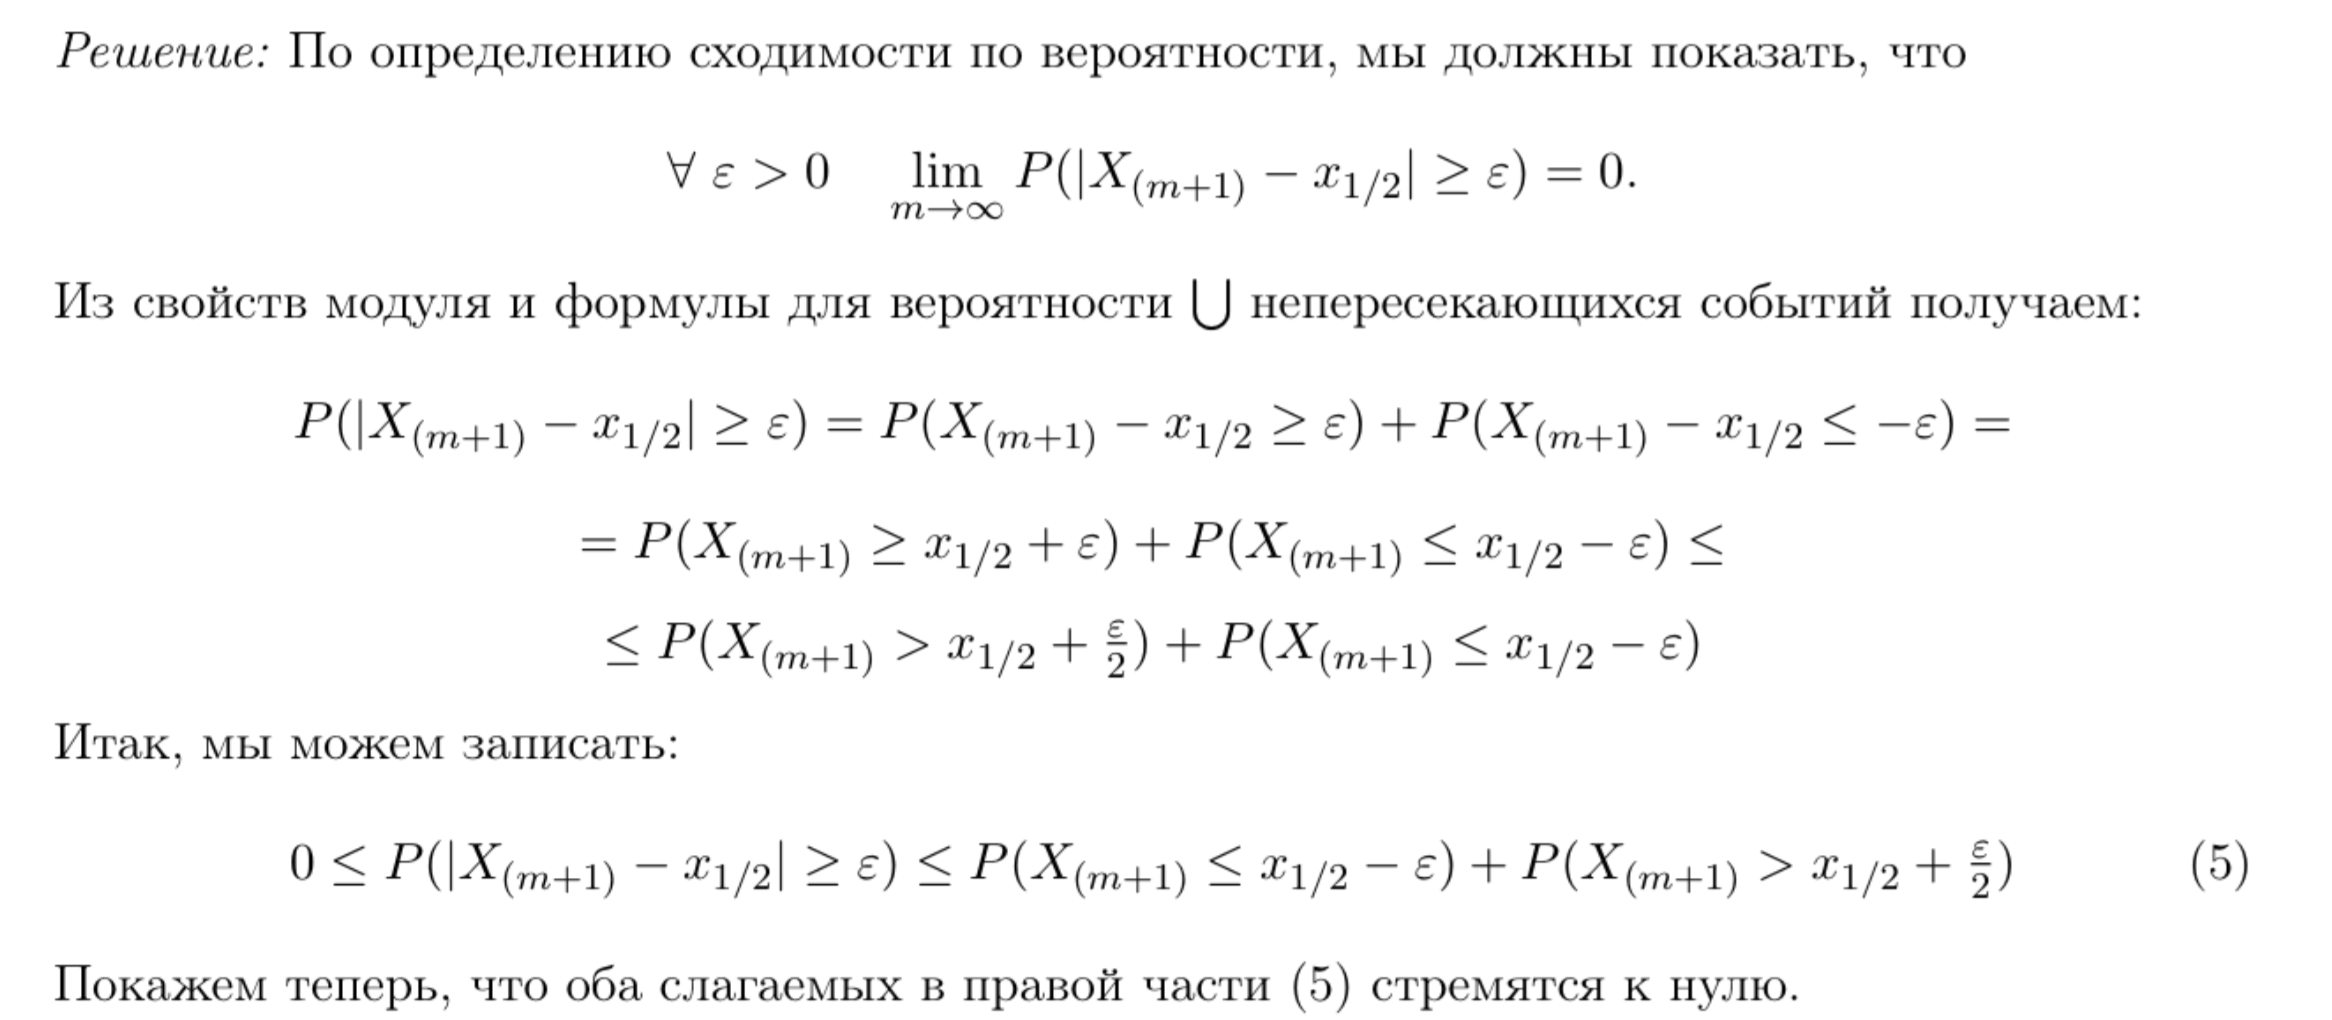
\includegraphics[scale=0.4]{1.png}
\end{center}
Применим представление с семинара:
\[
P \left(
X_{(m + 1)} \leq x_{\frac12} - \varepsilon \right) = 
P \left( 
\sum_{j = 1}^{2m} Y_{j}^{t_1} \geq m + 1
\right)
\]
Где $t_1 = (x_{\frac12} - \varepsilon)$, а величины $Y_1^{t_1}, \ldots Y_{2m}^{t_1}$ -- результаты $n$ независимых испытаний с вероятность успеха $p_{t_1} = F_{X_1}(t_1)$ и вероятностью неудачи $q_{t_1} = 1 - F_{X_1} (t_1)$. Сделаем следующее преобразование выражения под знаком вероятности:
\[
P \left( 
\sum_{j = 1}^{2m} Y_{j}^{t_1} \geq m + 1
\right) = P \left(
\frac{\sum Y_j^{t_1} -(2m) \mathbb{E}Y_1^{t_1}}{\sqrt{2m + 1} \sqrt{\mathbb{D}Y_1^{t_1}}}
\geq \frac{m + 1- 2m \mathbb{E} Y_1^{t_1}}{\sqrt{2m} \sqrt{\mathbb{D}Y_1^{t_!}}}
\right)  
\]
Из ЦПТ можно вывести, что при $m \rightarrow \infty$:
\[
P \left(
\frac{\sum Y_j^{t_1} -(2m) \mathbb{E}Y_1^{t_1}}{\sqrt{2m + 1} \sqrt{\mathbb{D}Y_1^{t_1}}}
\geq \frac{m + 1- 2m \mathbb{E} Y_1^{t_1}}{\sqrt{2m} \sqrt{\mathbb{D}Y_1^{t_!}}}
\right)   
\sim \int\limits_{A_m}^{+\infty} \rho_{N(0, 1)} (t) dt
\]
Где:
\[
A_m = \frac{m + 1 - 2m \mathbb{E}Y_1^{t_1}}{\sqrt{2m} \sqrt{\mathbb{D} Y_1^{t_1}}} 
\]
Заметим, что $\mathbb{E} Y^{t_1} = p_{t_1}$, а $\mathbb{E} Y^{t_1} = p_{t_1} \cdot q_{t_1}$, поэтому:
\[
A_m = \frac{m(1 - 2p_{t_1}) - p_{t_1}}{\sqrt{2m} \sqrt{p_{t_1} \cdot q_{t_1}}}
\]
\begin{center}

\includegraphics[scale=0.7]{2.png}

\includegraphics[scale=0.5]{3.png}
\end{center}
\[
P\left(X_{(m + 1)} > x_{\frac12} + \frac{\varepsilon}{2}\right) = 1 - P\left(X_{(m + 1)} \leq  x_{\frac12} + \frac{\varepsilon}{2}\right) 
\]
Также:
\[
P\left(X_{(m + 1)} \leq  x_{\frac12} + \frac{\varepsilon}{2}\right)  = P \left(
\sum_{j = 1}^{2m} Y_j^{t_2} \geq m + 1
\right) \sim \int\limits_{B_m}^{+\infty} \rho_{N(0, 1)} (t) dt 
\]
Где $t_1 = x_{\frac12} + \frac{\varepsilon}{2}$, величины$Y_1^{t_2}, \ldots Y_{2m}^{t_2}$ -- результаты $n$ независимых испытаний с вероятность успеха $p_{t_1} = F_{X_1}(t_t)$, а число $B_m$ вычисляется как:
\[
B_m = \frac{m + 1 - (2m) \mathbb{E} Y_1^{t_2}}{\sqrt{2m} \sqrt{\mathbb{D} Y_1^{t_2}}} 
\]
Заметим, что $\mathbb{E} Y^{t_2} = p_{t_2}$, а $\mathbb{E} Y^{t_2} = p_{t_2} \cdot q_{t_2} = p_{t_2} (1 - p_{t_2})$. Поэтому:
\[
B_m = \frac{m(1 - 2p_{t_2}) - p_{t_2}}{\sqrt{2m} \sqrt{p_{t_2} \cdot q_{t_2}}}
\]
Поскольку $p_{t_2} = F_{X_2} (t_2) = F_{X_1} (x_{\frac{1}{2}} + \frac{\varepsilon}{2})$ , из задачи 4 следует, что:
\[
p_{t_2} = F_{X_1} (x_{\frac12} + \frac{\varepsilon}{2}) > F_{X_1} (x_{\frac12}) = \frac12 
\]
Формула для $B_m$ и неравенство $p_{t_2} > \frac12$ гарантируют, что $B_m \overset{m \rightarrow \infty}{\longrightarrow} -\infty$, поэтому:
\[
P\left(X_{(m + 1)} \leq  x_{\frac12} + \frac{\varepsilon}{2}\right)  \rightarrow 1
\]
\[
P\left(X_{(m + 1)} > x_{\frac12} + \frac{\varepsilon}{2}\right) = 1 -  P\left(X_{(m + 1)} \leq  x_{\frac12} + \frac{\varepsilon}{2}\right)  \rightarrow 0 a
\]
Итак, мы показали, что $P\left(X_{(m + 1)} > x_{\frac12} + \frac{\varepsilon}{2}\right)$ и $P\left(X_{(m + 1)} \leq  x_{\frac12} - \varepsilon \right)$ стремятся к нулю, вспомним неравенство из самого начала решения:
\[
0 \leq P \left(
|
X_{(m + 1)} - x_{\frac12} 
| 
\geq \varepsilon
\right)
\leq 
P\left(X_{(m + 1)} > x_{\frac12} + \frac{\varepsilon}{2}\right) + P\left(X_{(m + 1)} \leq  x_{\frac12} - \varepsilon \right) 
\]
Благодаря теореме о зажатой последовательности мы получаем, что $P(|X_{(m + 1)} - x_{\frac12}| \geq \varepsilon)$ стремится к нулю при $m \rightarrow \infty$, отсюда и следует сходимость $X_{(m + 1)} \overset{P}{ \rightarrow } x_{\frac12}$ при $n = 2m \rightarrow \infty$. Аналогично доказывается для $X_{m}$. А значит получаем то, что хотели
\begin{center}
\textbf{Ч.Т.Д} 
\end{center}
\clearpage
\section*{Задача 11 [листок 6]}
\[
\begin{cases}
\varrho(x) = e^{-(x - a)}, \; x > a \\
\varrho(x) = 0,  \; x \leq a
\end{cases}
\]
Используем метод момента:
\[
\mathbb{E} X = \int\limits_{-\infty}^{+\infty} x \cdot e^{-(x - a)} \cdot I_{x  > a}   dx = \int\limits_{a}^{+\infty} x \cdot e^{-(x - a)}  dx = -x \cdot e^{-(x - a)} \Bigg|_a^{+\infty} + \int\limits_a^{+\infty} e^{-(x - a)} dx = a + 1
\]
Значит:
\[
\overline{X} = a + 1  \rightarrow a = \overline{X} - 1
\]
\begin{center}
\textbf{Ответ: } 
\[
a = \overline{X} - 1
\]
\end{center}
\end{document}
